%----------------------------------------------------------------------------------------
%	PACKAGES AND OTHER DOCUMENT CONFIGURATIONS
%----------------------------------------------------------------------------------------

\documentclass[12pt, titlepage, reqno]{article} % Document font size and equations flushed left
 \usepackage[super,sort&compress]{natbib}
 \usepackage{amssymb, latexsym}
 \usepackage{amsmath} 
 \usepackage{amsthm}
 \usepackage{bm}
 \usepackage[mathscr]{eucal}
 \usepackage{enumerate}
\usepackage{url}
\usepackage{graphicx}% http://ctan.org/pkg/graphicx
\usepackage{color}
\renewcommand{\thefootnote}{\alph{footnote})}    
 \renewcommand{\baselinestretch}{2}
 \renewcommand{\section}[1]{\medskip \addtocounter{section}{1}\raggedright 
     \textbf{\Roman{section}. \ #1}\medskip \setcounter{subsection}{0}
    \setlength{\parindent}{5ex}
 }
 \renewcommand{\subsection}[1]{\medskip \addtocounter{subsection}{1}\raggedright
    \textbf{\Alph{subsection}. \ #1} \medskip \setcounter{subsubsection}{0}\setlength{\parindent}{5ex}
}
 \renewcommand{\bibsection}{\medskip \raggedright  \textbf{REFERENCES}
    \medskip}
 \renewcommand{\bibnumfmt}[1]{\textbf{{#1}.}\ \ }
 \pagestyle{myheadings}
 \markboth{\hfill Lafay et al., JASA, p.\ }{\hfill Lafay et al., JASA, p.\ }
 \setlength{\parindent}{5ex}
 
 \setlength{\paperwidth}{8.5in}
 \setlength{\textwidth}{6.5in}
 \setlength{\oddsidemargin}{0in}
 \setlength{\evensidemargin}{0in}
\usepackage{setspace}
\usepackage[format=hang,font={scriptsize,onehalfspacing},labelfont=bf]{caption}

\begin{document}
\begin{titlepage}

 \begin{center}

 \textbf{Approaching mental representations of urban soundscape using auditory scenes simulation}\\
 
 
 
 \vspace{10ex}

\textbf{Gr\'egoire Lafay\footnote{e-mail: gregoire.lafay@irccyn.ec-nantes.fr}, Mathieu Lagrange and Jean-Fran\c cois Petiot}\\

Institut de Recherche en Communications et  Cybernétique de Nantes (IRCCYN) \\

Ecole centrale de Nantes, France \\

\textbf{Mathias Rossignol and Nicolas Misdariis }\\

Institut de Recherche et Coordination Acoustique/Musique (IRCAM) \\ 

Paris, France \\

\textbf{pacs: 43.50.Lj, 43.50.Rq, 43.50.Qp, 43.66.Lj, 43.66.Ba}
 \end{center}

 \end{titlepage}


%\renewcommand{\baselinestretch}{1}

%----------------------------------------------------------------------------------------
%	ARTICLE INFORMATION
%----------------------------------------------------------------------------------------

%




%\title{Approaching mental representations of urban soundscape using auditory scenes simulation}
%\author{Grégoire Lafay}
%\affiliation{Institut de Recherche en Communications et  Cybernétique de Nantes (IRCCYN), Ecole centrale de Nantes, France}
%\author{Mathias Rossignol}
%\affiliation{Institut de Recherche et Coordination Acoustique/Musique (IRCAM), France}
%\author{Nicolas Misdariis}
%\affiliation{Institut de Recherche et Coordination Acoustique/Musique (IRCAM), France}
%\author{Mathieu Lagrange}
%\affiliation{Institut de Recherche en Communications et  Cybernétique de Nantes (IRCCYN), Ecole centrale de Nantes, France}
%\author{Jean François Petiot}
%\affiliation{Institut de Recherche en Communications et  Cybernétique de Nantes (IRCCYN), Ecole centrale de Nantes, France}

\begin{abstract}
This paper introduces a subject-centered experimental protocol to study mental representations of urban soundscapes through a simulation process. Subjects are asked to recreate a full sound environment by means of a structured sound data set and a  software dedicated to sound manipulation. This paradigm is used to characterize urban sound environment representations, by analyzing the sound classes that were used to simulate the auditory scenes. Results show that a semantic characterization in terms of presence~/ absence of sound sources is an effective way to characterize urban sound environments.
\end{abstract}


%\maketitle % Print the title and abstract box

%%%%%%%%%%%%%%%%%%%%%%%%%%%%%%%%%%%%%%%%%%%%%%%%%%%%%%%%%%%%
%%%%%%%%%%%%%%%%%%%%   INTRODUCTION     %%%%%%%%%%%%%%%%%%%%
%%%%%%%%%%%%%%%%%%%%%%%%%%%%%%%%%%%%%%%%%%%%%%%%%%%%%%%%%%%%

 \addtocounter{page}{2}

 \section{Introduction}
 
 \setlength{\parindent}{5ex}


The notion of soundscape has been introduced by Schafer \cite{schafer_new_1969, schafer1977tuning} in the 1970s as the auditory equivalent to landscape. Following this paradigm, a sonic environment is described by focusing on the listener's evaluation, rather than only taking into account the acoustic parameters of the sound. Focusing on subjective criteria, Schafer proposed to decompose the soundscape between three main components called \textit{keynote sounds}, \textit{signals} and \textit{soundmarks}. The notion of soundmark refers to sounds with subjective qualities that bring them into focus for a certain category of people, whereas keynote sounds and signals may roughly be considered as respectively background and foreground sounds. Schafer also claims that the improvement of the sonic environment requires a ``\,positive\,'' approach to the soundscape, involving the identification and reinforcement of pleasant, important or meaningful sounds in the environment. The soundscape thus appears as a powerful tool to develop perceptively motivated acoustical indicators \cite{schulte-fortkamp_soundscape:_2007}.



The main goals of studies addressing soundscape perception may be summarized as follow:

\begin{enumerate}
\item \textit{Describing the soundscape}: How does the human brain identify different types of soundscapes? What are the elements composing each type of soundscape? How do they differ from one soundscape type to another? 
\item \textit{Evaluating the soundscape}: How do those elements influence the qualitative evaluations of a soundscape, such as ``\,noise annoyance\,'' or ``\,pleasantness\,'', to name but a few?
\end{enumerate}

The second question finds its origin in the growing need to improve the quality of artificial sonic environments, such as the urban soundscape. It is only during the 1980s that policy-makers started taking into account the link between \textit{noise} and pollution, considering noise as a significant degradation of the quality of life. To fight this pollution, the first approach consisted in identifying unwanted sounds, and lowering their intensities. Thus, in the wake of this realization, several regulations have emerged, often limited to enforcing sound level thresholds. However, several studies showed that urban ``\,noise\,'' perception and evaluation is a complex phenomenon that cannot be described solely with the help of objective acoustical measures such as A-weighted levels and $L_{Aeq}$ \cite{schulte-fortkamp_soundscape_2006, schulte2013soundscape,dubois2006cognitive,dubois2000categories,raimbault_urban_2005,guastavino_etude_2003}. More precisely, Yang and Kang \cite{Yang2005211} as well as Kang and Zhang \cite{kang_semantic_2010} found significant differences between objective acoustic comfort measurements and subjective evaluations of sonic environments, thus confirming that ``\,noise\,''  is a cognitive object which depends on a listener's appreciation and the context in which the noise is heard. Many urban ``\,noises\,'' such as that of a \textit{siren}, can annoy as well as warn of a danger. Many town districts are appreciated because of their lively and animated atmosphere which often results in higher sound levels. 



To summarize, we believe that even if acoustical regulations  are to some extent effective, there is a need to describe urban soundscapes not only through objective acoustical measures. Qualitative attributes also need to be considered \cite{torija2013application, cain_development_2013} in order to understand better the relationship between humans and their acoustic environment\cite{schafer1977tuning}. 

\section{Background}

The strength of the soundscape approach is, to some extent, also its weakness, as it implies to  fully appreciate the interaction of many factors. Perception of soundscape is thus an interdisciplinary field of investigation, each discipline coming with its well identified experimental protocol. In each one, integration of the results can be difficult \cite{davies_perception_2013, schulte-fortkamp_soundscape:_2007}. Recently, ambitious projects have been undertaken as the European Cooperation in Science and Technology Action TD0804-Soundscape of European Cities and Landscapes to standardize soundscape assessment and indicators. 

We believe that studies addressing soundscape perception may be roughly divided into two approaches according to their methodologies \cite{davies_perception_2013}. 

The first approach is the dimensional approach, which tends to derive relevant emotional dimensions using semantic differential analysis  \cite{cain_development_2013, jeon2013soundwalk, kang_semantic_2010}, and to link those dimensions with acoustical descriptors \cite{torija2013application}. The idea is to investigate the soundscape using both acoustical measurements and semantic data.  In order to establish the semantic axis \cite{davies_perception_2013} prior to the dimensional analysis, those semantic data usually come from qualitative surveys. Using a Principal Component Analysis (PCA) on descriptors of urban soundscapes, Cain and al.\citep{cain_development_2013,davies_perception_2013} found two independent emotional dimensions named ``\,Calmness\,'' and ``\,Vibrancy\,''.  Using a hierarchical cluster analysis on both semantic differential attributes and acoustical descriptors, Torija and al. \cite{torija2013application}  derive 15 soundscape typologies and show that crest factor and sound level at 125Hz are relevant acoustical variables to recognize types of soundscape. Although the dimensional approach provides important cues to describe soundscape perception, it remains a purely holistic approach as it bypasses the way in which the human brain decomposes soundscapes into perceptual auditory objects \cite{bregman1994auditory, winkler2009modeling} and how each of those objects may influence the qualitative judgment. 

The second approach is the categorical approach, which investigates mental representations of soundscape. Mental representations can be seen  as mirrors of the perceived external realities (see Dubois et al. \cite{dubois2006cognitive} p.869 for a definition). They are the memory of the knowledge acquired by a subject, and act as the base of \textit{top-down } cognitive systems. As explained by Dubois et al.  \cite{dubois2006cognitive} ``\,semantic categories can be seen as mediating individual sensory experiences to collective representations by means of a shared language\,''. As they cannot be observed, experimenters must use objectivation methods to reach them. Traditional methods used to objectify human mental representations attempt to derive mental categories and perceptual components, either by relying on verbal descriptions coming from questionnaires or interviews \cite{raimbault_urban_2005, guastavino_ideal_2006, axelsson2005soundscape} (categories of sound sources) or by sorting tasks \cite{guastavino_categorization_2007, maffiolo_caracterisation_1999, houix_lexical_2012} (categories of sound sources and soundscapes).  To identify the mental categories, these methods require psycho-linguistic and lexical analyses. Results from those studies tend to show that the soundscape appreciation depends upon the identification and the assessment of the sound sources which compose the soundscape \cite{raimbault_urban_2005, maffiolo_caracterisation_1999, dubois2006cognitive, guastavino_ideal_2006, guastavino_categorization_2007}. The categorical approach thus agrees with the Auditory Scene Analysis (ASA) theory \cite{bregman1994auditory}, which stands that auditory stimuli are decomposed into ``\,auditory objects\,'' called ``\,streams\,'', which may be regarded as sequences of auditory events emitted by putative sound sources \cite{ciocca2007auditory,winkler2009modeling}. This view is in line with recent cognitive neuroscience studies suggesting that the primary auditory cortex (A1) produces representations of such auditory objects that act as bases for high level cognitive processing \cite{nelken2008neurons}.

As underlined by Davies and al. \cite{davies_perception_2013}, while the categorical approach provides useful information to understand how a soundscape is composed, it does not provide information on how the relations (acoustic or semantic) between the soundscape components (sequences of audio events emitted by sound sources) are perceived and influenced the qualitative evaluation. Furthermore, as category ``\,names\,'' may occur at different semantic levels, categorical approaches based on linguistic analysis are not amenable to facilitating comparison between studies \citep{niessen_categories_2010, brown_towards_2011}. To go further in the categorical approach, there is a need for methods  providing 1) a finer characterization of sound source categories with semantic and numeric data, 2) a description of the inter-relations existing between these sound sources, and 3) subjective data that may be used as basis for inter-studies comparisons.

\section{Method overview}

With those considerations in mind, we propose a new  subject-centered experimental protocol to characterize sound environments with qualitative data related to quantitative data. In this protocol, subjects are asked to simulate complex sound environments with pre-imposed associated qualitative appreciations. To do so, they have access to a soundscape simulator that uses classes of sounds as base elements. The soundscape simulator is thus bound to a sound data set of urban environmental sounds, organized hierarchically around sound categories found in previous studies \cite{maffiolo_caracterisation_1999,dubois2006cognitive, guastavino_categorization_2007, guastavino_ideal_2006, niessen_categories_2010, brown_towards_2011}. The proposed protocol was previously tested and validated thanks to a pilot study\cite{soundscape3} with 10 subjects.

Previous works done by Bruce et al. also use a soundscape simulator to study soundscape perception \cite{bruce2009development,bruce2014effects}. But in their approach, subjects may only add or remove a short set of long recordings of foreground sounds, and adjust their levels. In our approach, subjects are presented with a full data set of classes of urban environmental sounds, that they may manipulate in terms of sound intensity and time positioning.

The proposed protocol is used to characterize two antagonistic soundscapes: subjects are asked to simulate two full urban sonic environments, one ``\,ideal\,'' and the other ``\,non-ideal\,''. The names ``\,ideal\,'' and ``\,non-ideal\,'' have been chosen in order to compare the results with those of a previous study addressing ideal urban sound environment representations \cite{guastavino_ideal_2006}. In this paper, the focus is put  on the acoustical analysis of the simulated scenes to figure out what the characteristics of an ideal (resp. non-ideal) urban environment are, in terms of sound source composition, sound event densities and sound levels. To refine the analysis, sound sources categories and their related quantitative data are investigated according to different semantic levels of categorization (\textit{urban transport}$>$\textit{car}$>$\textit{car-passing}) \cite{niessen_categories_2010, brown_towards_2011}.

The simulated scenes as well as the annotations are available on the archive Data Repository: \url{https://archive.org/details/soundSimulatedUrbanScene}
The experiment web-page is available via the link \url{http://soundthings.org/simScene/}. It should be run on the Chrome browser or the Mozilla Firefox browser.

\section{Experimental paradigm}

The proposed experimental protocol is largely inspired  by hypotheses coming from cognitive psychology\cite{dubois2000categories,dubois2006cognitive} and categorization theory \cite{roach1978cognition}. A sound is considered both for its physical properties and for its semantic value which both depend on the subject and the context (urban environment). The purpose of our  protocol is to objectify human mental representations of the sonic world without the need for a linguistic analysis, by characterizing them with combined semantic and numerical data.

To that end, subjects are asked to recreate a complex sound environment, making use of an environmental sound data set that they may explore without any written textual help thanks to a selection interface designed for this study. The selection process  has been designed to rely only on the listening of sounds themselves, in order not to influence subjects with \textit{a priori} associated semantic values. Once a sound element is selected, subjects must name it. They may then modify some of its physical parameters, thanks to a set of audio controllers.  This framework is depicted on Figure~\ref{Paradigm}. It exposes three types of data to objectify mental representations:

\begin{enumerate}
\item  \textit{Generic semantic data}: the ``\,tags\,'' of the sounds chosen by the subject. A tag is relative to the nomenclature of our typology, and thus pre-defined by experimenters. (ex: \textit{male-voice})
\item \textit{Quantitative data}: the set of ``\,audio parameters\,'' attributed to the sounds by the subject (ex: \textit{sound level} dB).
\item \textit{Non-generic semantic data}: all the subjective verbal data including  the \emph{names} given by the subject to the sounds they selected (ex: \textit{the cries of a man}), a general \emph{title} of the simulated scene, and a \emph{free comment} concerning the creation process.
\end{enumerate}

The proposed paradigm can thus be seen as the inverse of that of a description task (questionnaire, interviews) that uses audio data as input (see Figure~\ref{psycholing}). In contrast with interviews and questionnaires, which both require subjects to describe a soundscape, \textit{i.e.} to decompose the soundscape in elements, subjects are asked to recompose the soundscape from a sound data set of urban environmental sounds. This sound data set  represents the ``\,sonic world\,'': a semantic discretization of it in term of  ``\.sound sources\,''. It ideally  provides the subject with all the sound diversity he may desire. 

The proposed approach questions the following: ``\,What sounds have been \emph{used}?\,'', ``\,how have they been \emph{used}?\,'' and  ``\,how have they been \emph{named}?\,'', whereas descriptions  tasks respond to:  ``\,What sounds have been \emph{named}?\,'' and ``\,how have they been \emph{described}?\,''.

\begin{figure}[t]
\begin{center}
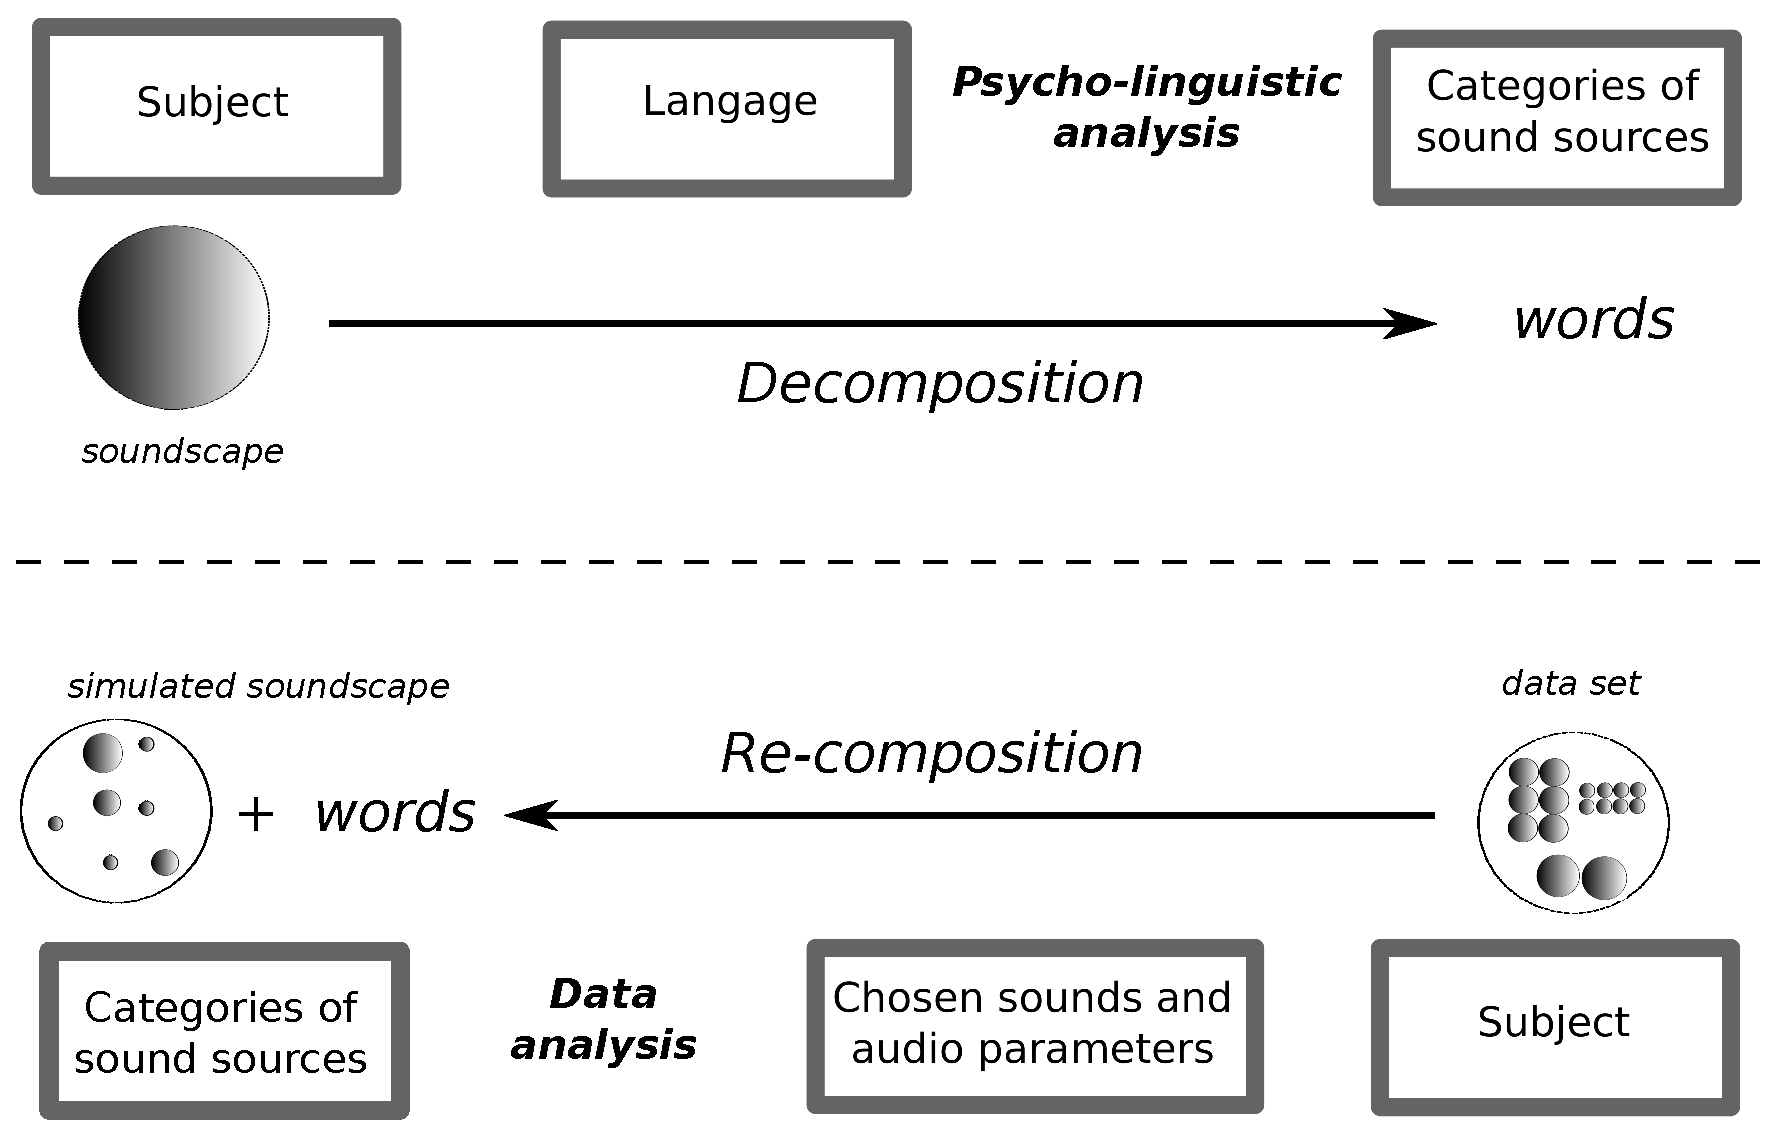
\includegraphics[scale=1]{1.eps}
  \caption{\label{psycholing} Sketch illustrating the psycho-linguistic analysis paradigm (top) and the proposed approach (bottom)}
  \end{center}
\end{figure}


 \begin{figure*}[t]
\begin{center}
\includegraphics[scale=1]{2.eps}
  \caption{\label{Paradigm} Sketch illustrating the paradigm of the proposed experimental protocol. \textit{square}: non-generic semantic data; \textit{star}: generic semantic data; \textit{circle}: audio and quantitative data; \textit{Dashed-line}: data not addressed in this paper; \textit{Line}: data addressed in this paper}
  \end{center}
\end{figure*}

\section{Simulating the soundscape}

\subsection{Soundscape model}


In order to allow the creation of a complex sound environment, a model of soundscape has been designed whose key aspects are now presented. A soundscape is assumed to be a sum of tracks. Each track is modeled by a temporal sequence of sound samples that belong to the same sound class. To this sense, each track is related to one specific sound class (leaf sound class more specifically, see \ref{subsection:Sound dataset}). To generate a soundscape, subjects may interact with the tracks, but not with specific sound samples. In other words, if a subject wishes to put a sequence of car sounds, he may choose the sound class \textit{car passing} and manipulate its associated track, but he cannot interact with individual sound samples of \textit{car passing}.

Concerning the sound classes, the commonly accepted distinction made between ``\,sound events\,'' and ``\,sound textures\,''  is taken into account. A  soundscape  is thus regarded as  ``\,a skeleton of events on a bed of texture\,'' \cite{nelken_ear_2013}. Several studies point out the fact that textures and events drive two distinct cognitive processes \cite{maffiolo_caracterisation_1999, saint-arnaud_classification_1995, mcdermott2013summary}. If there is to some extend an analogy between the  notion of ``\,sound event\,'', and the Schaferian notion of ``\,signal\,'', the analogy is not obvious between the notions of ``\,texture\,'' and keynote. Schafer's definition of keynote is perceptively motivated whereas most  definitions of texture  adopt a morphological approach (see \cite{saint-arnaud_classification_1995} for a definition of texture, which is the one adopted in this paper).

Following this distinction (events \textit{vs} textures), two separate treatments are handled by the soundscape simulator:

\begin{itemize}
\item \textit{For the sound event classes} the temporal sequence is made of randomly selected sound samples belonging to the considered sound class of events. the temporal sequence is scaled by the mean/average spacing time between the sound events, the beginning and the end of the sequence.
\item \textit{For the sound texture classes} the temporal sequence is made of randomly selected texture samples belonging to the considered texture class, which are sequenced without time space (crossfading is used to guarantee that the transition is seamless). Only the beginning and the end of the sample sequence may be set by the subject. Furthermore, in order to avoid any unnatural effect due to the repetition of identical sounds \cite{agus_rapid_2010}, the soundscape simulator guaranties that a sample will never transition to itself.
\end{itemize} 

Six audio parameters allow the subject to manipulate sound sequences of each selected class, in terms of sound levels and time positioning, see Table~\ref{Audio parameters}. The parameters have an effect on all the samples of a sound sequence. To this sense, sound levels, and time spaces between events (only for events classes) are controlled in terms of average and variance between all the sound samples. Global parameters as global fade in/out and start/stop positions act on all the sequence. A last parameters called ``\,sample fade in/out\,'' allows subject to set a same fade effect separately on each sample of an events sequence (only for events classes).


\subsection{Sound data set}
\label{subsection:Sound dataset}

Segmenting the sonic world to provide the subject with a reasonable and representative number of sound events and textures is a crucial step of our experiment. In order to create our sound data set, we rely on previous studies addressing urban sound source categories\cite{maffiolo_caracterisation_1999, dubois2006cognitive,guastavino_categorization_2007, guastavino_ideal_2006, niessen_categories_2010, brown_towards_2011}. Based on the names of those categories, we build two hierarchical structures of event and texture sound classes,  respectively. Top classes of those structures represent concepts as ``\,urban transport\,'' grouping  sound classes such as ``\,boat\,'' or  ``\,cars\,'', which are themselves grouped in sub-classes. The deeper the class level, the lower the variability between the exemplars lying under the class. In this paper, the class levels will be referred as \textbf{semantic levels}, the top classes being at the semantic level 0, the first subclasses at the semantic level 1 and so forth until the leaf classes are reached. Leaf classes are collections of recorded sound samples. Subjects may only interact with the leaf classes. The Figure \ref{datasetexample} illustrates the hierarchical structure.

\subsection{Simulation process}
The simulation process involves two steps (see Figure~\ref{task}), each of them relying on particular data resources and software interfaces. The two steps are: 

\begin{enumerate}
\item \textit{Sound Class selection}: where the subject has to select a leaf class of sound (``\,car passing\,'', ``\,heavy rain\,'', \ldots{}).  The sele	ction is made without any written verbal help thanks to a particular selection interface.
\item \textit{Sound Class modification}: where the subject may tune the parameters (time and intensity) of the temporal sequence formed by sounds belonging to the selected sound class.
\end{enumerate}
 



%%%%%%%%%%%%%%%%%%%%%%%%%%%%%%%%%%%%%%%%%%%%%%%%%%%%%%%%%%%%
%%%%%%%%%%%%%%%%%%%%   METHODOLOGY     %%%%%%%%%%%%%%%%%%%%%
%%%%%%%%%%%%%%%%%%%%%%%%%%%%%%%%%%%%%%%%%%%%%%%%%%%%%%%%%%%%

\section{Experiment}
\subsection{Participants}
44 post-graduate students of the {\'E}cole Centrale de Nantes (French engineering school), were asked to take part in the experiment. They were 30 males and 14 females and were about the same age (M: 21.6, STD: 2). All of them have been living in the same large French city (Nantes) for at least two years.  

\subsection{Apparatus}
483 urban environmental sounds were collected, of which 381 sound events and 102 textures. Among them, 260 events and 72 textures were recorded by the authors. The rest, which proved to be particularly difficult to record, came from existing sound banks. All recordings were performed using the shotgun microphone \textit{Audio Technica AT8035} connected to a \textit{ZOOM H4n} recorder. The use of a shotgun microphone allowed us to isolate as much as possible sound recordings from undesired events. All the sound were normalized to the same root mean square (RMS) level. The experiment was run simultaneously with the 44 subjects spread in three identical rooms with calm environment. Subjects were forbidden to talk to one another. Audio was presented diotically to each participant via \textit{BeyerDynamic DT 990 Pro} semi open headphones. Three experimenters were always present (one in each room) to give instructions and answer queries if needed, including explanations, software installation and warm up session. 


\begin{figure}[t!]
\begin{center}
\includegraphics[scale=1]{3.eps}
\caption{\label{datasetexample} Sketch illustrating  the hierarchical structure of both the event and texture data sets. Depending on the considered top class, there could be more than 3 semantic levels.}
\end{center}
\end{figure}
\subsection{Task}

Subjects are asked to successively create two urban soundscapes. The first must be ideal (\textit{ie} the favorite urban soundscape of the subject in which they would like to live), the second non-ideal (\textit{ie} the worst urban soundscape of the subject in which they would not like to live). They are asked to mimic a static listener. Subjects are absolutely not restricted in their design choices, but are forbidden to create physically impossible situations such as ``\,a dog barking every 10 milliseconds\,''. Each simulation involves six steps which are exposed in Figure~\ref{task}. At the start of the experiment, a small tutorial of 20 minutes has been planed in order to familiarize the subject with the software environment. The experiment is scheduled to last about two hours.


\subsection{Data collection and analysis}
\label{Data collection}
Four subjects were excluded from the analysis due to a  misunderstanding of the instructions or a failure to comply with the time limits. 40 subjects completed the experiment successfully, giving us 40 ideal urban auditory scenes (i-scenes) and 40 non-ideal urban auditory scenes (ni-scenes). 

The proposed experimental protocol generated a large range of data suggesting numerous avenues of investigations. We here choose to restrict ourselves to 1) the  analysis of the holistic properties of the created scenes such as sound levels, event density and diversity, and 2) a class wise analysis, \textit{i.e.} the analysis of the properties attached to each specific sound class, and a study of the distribution of the classes among the ideal and non ideal scenes. Other aspects are intentionally left for future research. Thus, among the collected data, we focus on 2 types of data: 1) the generic semantic data being the ``\,tags\,'' of the chosen sound classes, and 2) the quantitative data being the sound levels attached to the sound classes. For the holistic analysis, the data are averaged over the scenes, without looking at particular sound classes. For the class-wise analysis, the scene content is investigated with respect to the different sound classes used.

%%%%%%%%%%%%%%%%%%%%%%%%%%%%%%%%%%%%%%%%%%%%%%%%%%%%%%%%%%%%
%%%%%%%%%%%%%%%%%%%%   RESULTS   %%%%%%%%%%%%%%%%%%%%%%%%%%%
%%%%%%%%%%%%%%%%%%%%%%%%%%%%%%%%%%%%%%%%%%%%%%%%%%%%%%%%%%%%

\begin{figure}[t]
\begin{center}
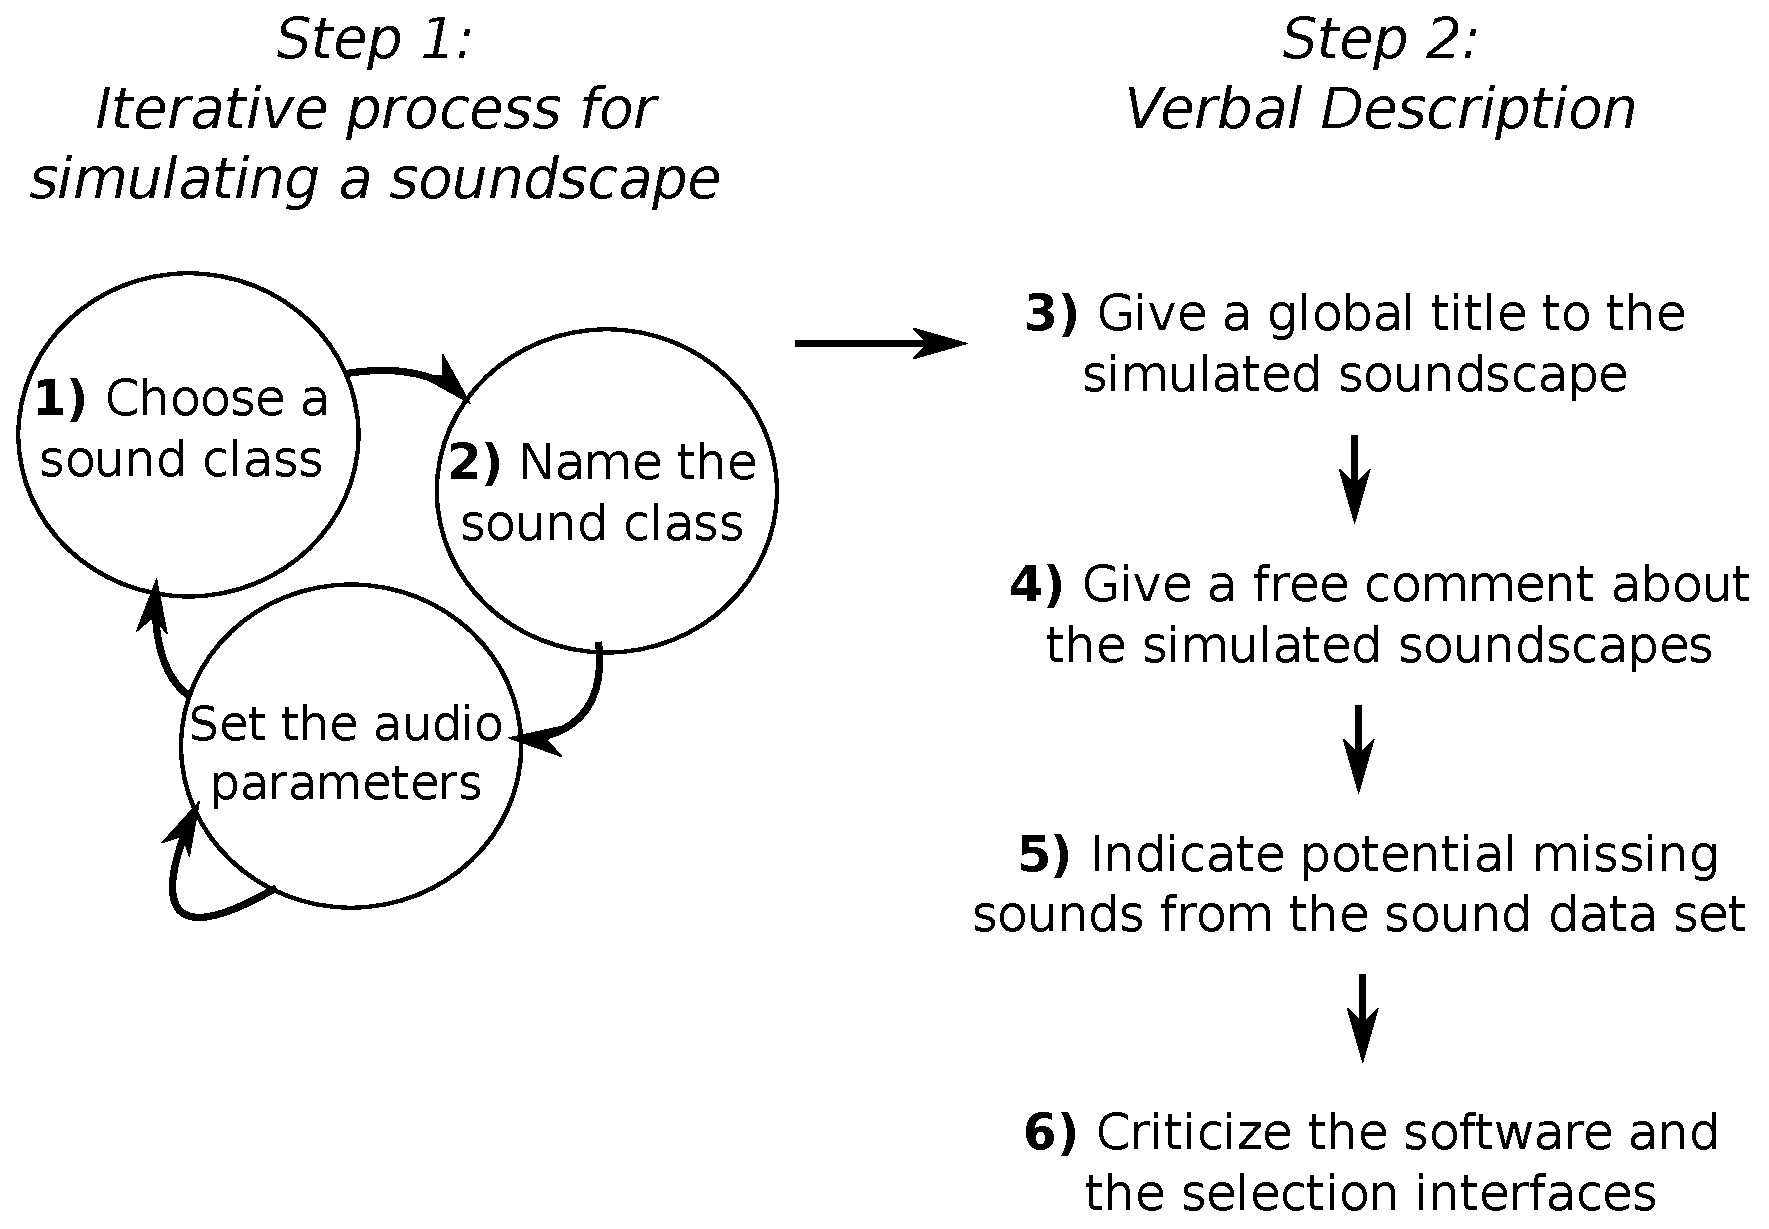
\includegraphics[scale=1]{4.eps}
  \caption{\label{task}Sketch illustrating the simulation process}
  \end{center}
\end{figure}

\section{Holistic analysis }

For the holistic analysis, all the statistical tests are performed using a Wilcoxon signed ranks test at the 5\% significance level. Observations are obtained by averaging the data related to each scene. Results are presented in the tables using the convention \textit{average(standard deviation)}.

\subsection{Sound levels}

Table~\ref{SNR} shows the results for the mean sound levels averaged over all subjects. For each scene, the mean sound level is obtained by averaging the sample levels. Samples are the elements which composed a temporal sequence of a particular sound class: if a subject selects the event sound class \textit{car passing} and creates a sequence  composed of 10 audio events, 10 samples are considered. This measure is thus not equivalent to the global sound level, but  can reasonably be considered a good indicator of the overall sound level of a scene.
Considering the event samples of the i- and ni-scenes, results show that the sound levels are significantly higher ($p=2.08*10^{-5}$) for the ni-scenes, indicating that sound levels are indeed on average higher for unpleasant sound environments. But if there is a blatant difference between the event sound levels of the i- and ni-scenes, the deviation between the texture sound levels is not significant($p=0.14$). This result suggests that textures have less direct influence on the sound level perception. This could be due to the fact that textures are sounds with low semantic weight \cite{saint-arnaud_classification_1995}, in other words, sounds which are less easy to identify. This is in line with early results of Kuwano et al. \cite{kuwano_memory_2003-1} showing that overall judgment of loudness of a sound environment sequence is not statistically different with average instantaneous judgment of the recalled sound events of the sequence.   




\subsection{Diversity and coverage}

The notion of diversity is addressed by observing the number of distinct sound classes (events and textures) used in each i- and ni-scenes. This number depends on the semantic level considered. For example, let us consider two ni-scenes, one having a sound class \textit{car-passing} of the semantic level 2, and the other a sound class \textit{car-starting}, also of the semantic level 2. Both classes  belong to the hierarchical structure \textit{transport} (level 0) $>$ \textit{car} (level 1). We will count 2 distinct sound classes for the semantic levels 2 and 3 (as \textit{car-starting} and \textit{car-passing} have no subclass), and only 1 sound class for the semantic levels 0 and 1. 

Averaged results  are shown in Table \ref{Diversity}. Except for the semantic level 0, the diversity is significantly higher for the ni-scenes (level 1: $p = 2.5*10^{-4}$;  level 2: $p =0.006$;  level 3: $p = 0.011$;). This reveals that ni-scenes are composed of a larger variety of sounds than i-scenes, suggesting that a non ideal urban environment contains more distinct sound sources than an ideal urban environment. 

To qualify this measure of diversity, and verify that it is not biased by the selection interface, we look at the coverage. The coverage is defined by the percentage of the sound classes (events and textures) of the data set that have been used by all the subjects. For example, if all the classes of the semantic level 1 have been chosen by at least one subject, the coverage for the semantic level 1 will be of 100\%. A low coverage would suggest that some parts of the data set have not been explored. Results are shown in Table \ref{Diversity}. The coverage remains superior to 85\% regardless the semantic level, indicating that most of the sounds have been used for each type of scenes. 





\subsection{Event density}

The event density is defined as the number of event sound samples used to generate a scene, regardless of the classes.  We can see that the numbers of sound samples vary widely with the subjects. There is no statistical difference between the densities of the i- and ni-scenes ($p=0.14$). This suggests that the global sound events density  does not influence the qualitative evaluation of a urban soundscape.

\section{Class-wise analysis}
For the class-wise analysis, all the statistical analyses are done using a Wilcoxon rank-sum test (Mann-Whitney-Wilcoxon test) at the 5\% significance level. Observations are obtained by averaging the data related to each class.

\subsection{Semantic features: an effective way to evaluate soundscape quality}
\label{Semantic Tag}

In order to describe the scenes in terms of sound sources, the ``\,tags\,''  of the sound classes (event and texture) chosen by the subjects are now investigated. Figures~\ref{tagI} and~\ref{tagNI} display the ``\,tags\,'' of the semantic levels 1 or 2. For ease of reading, the tags \textit{horn}, \textit{fire alarm} and \textit{car alarm} are grouped into a class named \textit{alarm/horn} the classes \textit{bus} and \textit{train} are grouped into a class named \textit{public transportation}, and the classes \textit{truck}, \textit{car}, \textit{scooter}, \textit{motorcycle} and \textit{start passage-way}  are grouped into a class named \textit{traffic}. Classes with a selection percentage less than 2 \% are not displayed.  We only count the selected sound classes and not the number of samples of their respective sequences.

There is considerable difference between the ``\,tags\,'' of the i- and ni-scenes, confirming that sound semantics play an important role in soundscape evaluation. To address this, each simulated scene is represented by a boolean vector of  $n$ dimensions $S_i = (x_1, x_2, \ldots{}, x_{n})$, $i\in[1,80]$. Each dimension corresponds to a sound class (event and texture) of a particular semantic level (for examples $n=44$ classes for the semantic level 1). Thus $x_1 = 1$ indicates that the sound class $x_1$ is present in the scenes $S_i$ (not present if $x_1=0$ resp.). A \textit{Jaccard} distance is then computed between the vectors $S_i$. To quantify how semantic features characterize both the i- and ni-scenes, the precision at rank 5 ($P@5$) metric is used, \textit{i.e.} the average number of items of the same class among the 5 closest items to a given seed item. For each scene $S_i$, $P@5$ is thus obtained by averaging the number of scenes having the same label as $S_i$ (i or ni) among the five scenes $S_j$ ($j=1,...,5$) that are closest to $S_i$. Results are then averaged over the scenes $S_i$ ($i=1, \ldots{}, 80$). 


Results are shown in Table~\ref{jaccardtable}. For the semantic level 1, a $P@5$ of 90\% is found, with a random threshold of 58\%. The deeper the hierarchical level, the higher the $P@5$. We find 92.25\% for semantic level 2 and 92.75\% for semantic level 3. This is a strong indicator that semantic values of sounds are good descriptors to distinguish between the i- and ni-scenes. To refine the analysis, the same test is run considering separately the sound textures and the events to describe the scenes (for the semantic level 1, events: $S_i \in  S_i = (x_1, x_2, \ldots{}, x_{31})$ and texture: $S_i \in  S_i = (x_{32},x_{33}, \ldots{}, x_{44})$). The $P@5$ achieved for the semantic level 1 of 91\% for the events and 78.5 \% for the textures demonstrate that sound events contribute more to the perception of soundscape quality than sound textures.  

\subsection{Hierarchical analysis of sound categories}


The sound classes showed in the Figures \ref{tagI} and \ref{tagNI} are close to those found by Guastavino \cite{guastavino_ideal_2006} in a psycho-linguistic study also addressing  ideal urban soundscape perception. Classes that suggest human presence and nature are the most present in i-scenes while classes referring to mechanical and construction work sounds are used for ni-scenes. This fact has been observed in other psycho-linguistic studies \cite{dubois2006cognitive, raimbault_urban_2005, guastavino_categorization_2007}. It confirms the \textit{biophilia} hypothesis that ``\,humans are attracted to nature\,'' (Wilson quoted by Guastavino \cite{guastavino_ideal_2006}). However some differences are to be noted. In her study, Guastavino \cite{guastavino_ideal_2006} point out that ``\,public transports\,'' are typical sounds of an ideal urban environment (also mentioned by Dubois et al. \cite{dubois2006cognitive}). She attributes this observation to the fact that urban environment perception is driven by the meaning attributed to the identified sources. As this meaning is influenced by social values, public transport sounds are better accepted than those of private vehicles. Our results tend to qualify this claim  by showing that sounds of public transports (\textit{bus} and \textit{train}) were chosen for both the i-scenes (3.97\% of the selected sound classes) and the ni-scenes (5.1\% of the selected sound classes). Moreover, the sound densities  (i-scenes: 1.1(2.1); ni-scenes: 1.4(2.2);  $p=0.2$) as well as the sample levels (i-scenes(dB): -1.5(3.1); ni-scenes(dB): -1.6(3.3);  $p=0.47$) do not differ significantly. Thus even if the idea of public transport sounds are well accepted due to societal considerations, the sound itself remains similar to that of any vehicles and appears in the ni-scenes more than \textit{car} or \textit{truck} sounds. Although semantic features influence the qualitative evaluation of public transport sounds (\textit{bus} sounds correspond indeed to 3.64\% of the event classes used in the i-scenes, as much as \textit{bicycle} sounds and more than any other vehicle sounds), it seems that, for this sound category, it is not predominant over the role played by the physical attributes of the sound. 

\begin{figure}[t!]
\includegraphics[scale=1]{5.eps} 
    \caption{\label{tagI}  Percentage of the number of sound classes of events (\textit{top}) and textures (\textit{bottom}) used by the subjects for the i-scenes at the semantic level 1 or 2 depending of the sounds}
\end{figure}
\begin{figure}[t!]
\includegraphics[scale=1]{6.eps}
    \caption{\label{tagNI}  Percentage of the number of sound classes of events (\textit{top}) and textures (\textit{bottom}) used by the subjects for the ni-scenes at the semantic level 1 or 2 depending of the sounds}
\end{figure}

Figures~\ref{tagI} and~\ref{tagNI}  indicate a counter-intuitive result showing that the event class \textit{traffic} (composed of the event subclasses \textit{truck}, \textit{car}, \textit{scooter}, \textit{motorcycle} and \textit{start passage-way}) is well represented in the i-scenes (10.3\% of the selected sound classes) as well as in the ni-scenes (21.6\%), thus suggesting that traffic sounds are an integral part of an ideal urban environment. If we look at the sample levels, there is no statistical difference between the i- and ni-scenes (i-scenes (dB): -1.8(2.1); ni-scenes (dB): -1.7(3.6); $p=0.17$). The difference occurs only if we look at the sample densities (i-scenes(dB): 2.7(4.5); ni-scenes (dB): 10.4(11.9); $p=3.6*10^{-5}$) which is significantly superior for the ni-scenes. These results tend to indicate that traffic sounds are not absent from the representation of an ideal urban environment provided their densities are not excessive. If we refine the analysis by assessing separately each event subclass of \textit{traffic}, we find significant differences only for the subclasses \textit{scooter} and \textit{motorcycle}. The former has a significantly higher density  ($p=5.6*10^{-4}$) for the ni-scenes, and the latter has both significantly higher sample levels ($p=0.03$) and density ($p=0.02$) for the ni-scenes. Putting these results with the urban problematic of ``\,traffic noise\,'', it appears that 1) it is mostly the sounds of two-wheeled vehicles that are the cause of the annoyance, and  2) that in this case, sound levels are not a relevant indicator of quality compared to sound density.


The texture class \textit{traffic hubbub} is well present in the i-scenes. There is no statistical difference between the i- and ni-scenes for both the sample levels ($p = 0.11$) and the densities ($p = 0.77$). Considering now the subclasses of  \textit{traffic hubbub} (see Figures \ref{tagI} and \ref{tagI}), we see that the \textit{Traffic hubbub of streets} class has been mostly used for the i-scenes (18.75 \% of the textures used in i-scenes) whereas  the \textit{Traffic hubbub of crossroad} class has been only used for the ni-scenes. If we compare those two subclasses, we find again no statistical differences for both the sample levels ($p = 0.19$) and the densities ($p = 0.37$).
These observations  show the importance of context and expectation in soundscape evaluation. The fact that \textit{traffic hubbub} is not depreciated for ideal urban environments shows that ``\,traffic sounds\,'' are understood as being an inherent element of urban environment. This is in contradiction with an intuitive idea that traffic background are indeed ``\,noises\,''. Similar findings are presented by Guastavino \cite{guastavino_etude_2003}: asking subjects to describe urban background, she found that appreciation of the \textit{traffic background} depends on the subject, as it can be reassuring or even appreciated, providing it is not too loud.


\subsection{Markers}



This section investigates the existence of potential event sound markers of an ideal urban environment (resp. non-ideal urban environment), \textit{ie} an event class which has been mostly used in one type of soundscape. To identify markers, the V-test statistical value is used. For each semantic level, considering the population as being  the total number  $n$ of event classes used for both i-scenes and ni-scenes, $n_k$ the number of event classes used for one type of scene $k$ (ni-scenes or i-scenes), $n_j$ the number of event classes $j$ used for both i-scenes and ni-scenes, and $n_{kj}$ the number of event classes $j$ used for one type of scene $k$ (ni-scene or i-scene), the V-test of the event class $j$ (modality) in the scene type $k$ (group) can be computed as follow:

\begin{align*}
\text{V-test}_{jk} = \dfrac{n_{jk} - n_k \frac{n_j}{n}}{\sqrt{n_k\frac{n-n_k}{n-1}\frac{n_j}{n}(1-\frac{n_j}{n})}} 
\end{align*}

The V-test tests the null hypothesis that the $n_k$ individuals of the group $k$ are randomly drawn from the population of $n$ individuals. Usually the V-test value is assessed at the 5\% significance level, that is, if the null hypothesis is true, the V-test value has a 95\% chance to fall within the confidence interval $[-1.96,1.96]$. Thus the V-test is considered as statistically significant if its absolute value remains superior to 2. It is safer to correct the usual 5\% significance level as we are testing many modalities (49 event classes for the third semantic level). To do so, we use the Bonferroni adjustment \cite{perneger1998s}. The Bonferroni adjustment is approximated by dividing the 5\% significance level by the number of modalities $j$ (event classes) to be tested. For example, if we test the 49 event classes of the semantic level 3, the corrected significance level will be 0.001\%, and the V-test value will be statistically significant if its absolute value is superior to 3.29.

Results are shown on the table \ref{table:markers}. Eleven markers are found across all the semantic levels. Confirming again the \textit{Biophilia} hypothesis, sounds of human (\textit{footsteps}, \textit{female laugh}, \textit{male laugh} and \textit{male footsteps concrete}) and nature (\textit{animal}, \textit{birds} and \textit{birds singing} ) are markers of the i-scenes. The presence of \textit{Church Bell} as a strong marker of the i-scenes can be due to the socio-cultural background of the subjects, in great majority French citizens. It confirms Schafer's claim that sounds that are recognized by a community as integral part of its sonic environment are popular \cite{schafer1977tuning}. 

For the ni-scenes, the markers  (\textit{Klaxon}, \textit{Siren}, \textit{vehicle work} and \textit{construction work}) are rather intuitive. Interestingly, none of the event classes related to traffic sounds is a marker of the i- or ni-scenes. It confirms the trend observed in \ref{Semantic Tag} that traffic sounds are understood to be intrinsically  part of a urban environment. In other words, although the event densities of traffic sound classes differ between the i- and ni-scenes, traffic sound classes presence is still not a characteristic of a non-ideal urban sound environment.


%%%%%%%%%%%%%%%%%%%%%%%%%%%%%%%%%%%%%%%%%%%%%%%%%%%%%%%%%%%%
%%%%%%%%    DISCUSSION AND PERSPECTIVES   %%%%%%%%%%%%%%%%%%
%%%%%%%%%%%%%%%%%%%%%%%%%%%%%%%%%%%%%%%%%%%%%%%%%%%%%%%%%%%%
\section{Discussion}
\subsection{About protocol validity}
One way to validate the protocol is to look at the subject comments. Looking at the database criticisms, 28 subjects stated that they couldn't find one or several desired sounds, with a maximum of 4 sounds for one subject. From all the missing sounds we identified 26 sound classes at different semantic levels. Among those classes, 16 were effectively present in the database, 1 referred to musical sounds which we had chosen to exclude from the database and only 9 were effectively absent. Among the 16 sound classes, they have all been used by at least one subject, except for one sound class (\textit{stroller/trolley}). Among the 9 missing ones, we find very specific sounds as \textit{sport car} or \textit{teenager voice}. We believe that those results show that the database diversity was sufficient for the purpose of the study.
If we look at the interface criticisms, 32.5 \% of all the subject clearly stood that the selection interface was a ``\,straightforward yet effective way\,'' to find a sound whereas  only 10 \% indicated that they encountered difficulties. The remaining 57.5 \%  did not report difficulties.  
Those results tend to confirm that both the data set and the selection interface are well suited for the experiment.

\subsection{Outcomes}


We believe that four main benefits may derive from using the proposed simulation approach: 1) Other studies based on description tasks use full  soundscapes recordings as input. Those recordings are specific exemplars of a very many potential soundscapes which could occur at the same location, at the same time. The re-composition process prevents experimenters from this bias as the simulated soundscape is directly related to the subject representation. Although the simulation is limited by the diversity of the sound data set, we believe that this bias is more controllable, as the expressiveness of the subjects' responses will be less constrained by the size of the data set  than by the exposure to imposed exemplars of a soundscape. 2) The presence of a structured sound data set allows us to focus directly on the sounds chosen by subjects instead of  verbal data only. Thus it may reduce the potential bias of a psycho-linguistic analysis, the first being the mastering of the subject's language by the subject, the second being the lack of definite terms to fully describe sounds or complex sound environments \cite{guastavino_ideal_2006}, and the third being the high inter-subject variability concerning the description of a same sound. 3)  The simulation protocol provides sound signals of simulated urban environments, annotated in term of sound sources, sound intensity, time positioning and qualitative appreciations. It allows us to appreciate new soundscapes descriptors as sample density, which otherwise would be tedious to obtain from recordings.

To some extend, those simulated scenes may be regarded as cognitive summaries of mental representations and may be a useful data set for all Computational Auditory Scene Analysis (CASA) research  or cognitive neuroscience studies investigating 'auditory object' decomposition \cite{nelken2008neurons} or regularities representation impact on high level perceptive processes\cite{winkler2009modeling}.

\section{Conclusions}

In this paper we introduced a new experimental protocol to study soundscape perception based on a simulation paradigm. Application of this protocol allows us to gain knowledge about the perception of urban soundscape by asking human subjects to simulate two urban sound environments: one ideal and the other non-ideal. The results of the presented study show that:

\begin{itemize}
\item The simulation paradigm provides the same high level sound categories as those observed by questionnaire based studies \cite{guastavino_ideal_2006}, and allows us to refine the hierarchical analysis of those sound categories.
\item A semantic characterization of the soundscape in term of presence~/ absence of sound sources is an effective way to characterize ideal or non-ideal urban environment.
\item Global sound level is indeed a good indicator of pleasantness, but not for specific sound categories.
\item Structural features such as sound event density are found to be relevant descriptors to characterize traffic sounds.
\end{itemize} 

These results indicate that associated semantic values of events is an effective information to categorize the simulated scenes between ideal and non ideal scenes. More precisely, the study shows that some event categories may be considered as markers of a specific type of soundscape. We believe that those results could be useful to guide the design of computational categorization paradigms based on automatic sound event detection.

We believe that this protocol allows us to directly objectify important aspects of the mental representations of the subjects by being able to look at 1) the sound classes chosen by the subjects to simulate the scenes and 2) their associated quantitative data.  Lastly, the use of a pre-fixed structured data set may facilitate the inter-subjects or inter-studies comparison as all subjects have access to the same decontextualized material to recreate their own vision (contextualisation) of a particular sound environment.  

We believe that performing this experiment with subjects of different socio-cultural backgrounds would be interesting for future work as it would allow us to study the cultural impact on the hearing cognitive processes involved.

 \noindent \textbf{Acknowledgements}
 
 \setlength{\parindent}{0.7cm} 

Research project partly funded by ANR-11-JS03-005-01. Thanks to the 44 students of the Ecole Centrale de Nantes for their willing participation.



%----------------------------------------------------------------------------------------
%	REFERENCE LIST
%----------------------------------------------------------------------------------------
\newpage
\bibliographystyle{unsrtnat}
\bibliography{biblio}


\newpage
 
 \begin{center}
 
 \large{Tables}
 
 
 \end{center}
 
\begin{table}[h]
\caption{\label{Audio parameters} Description of the audio parameters}
\begin{tabular}{l l} 
Audio Parameters & Description \\
\hline
Sound intensity (dB) & Average and variance \\
Spacing time (sec) & Average and variance \\
(only for event classes)&  \\ 
Position in Scene (sec) & Start and Stop\\
Fade In/out (sec)  & Global \\
Sample fade In/out (sec)  & For each events \\
(only for event classes)&  \\ 
\hline
\end{tabular}
\end{table}

\newpage
\begin{table}[h]
\caption{\label{SNR} Sound levels: mean sound levels in dB averaged over the subjects}
\begin{tabular}{l c c } 
              & Event classes & Texture classes\\
    \hline
	i-scenes & -6.8 (5.4) & -2.6 (3.9) \\
    ni-scenes& -2.4 (3.2) & -1.6 (2.6) \\
    \hline
\end{tabular}
\end{table}

\newpage
\begin{table}[h]
 \caption{\label{Diversity} Diversity and coverage: the coverage is the percentage of the sound classes (events and Textures) of the data set that have been used by all the subjects. The diversity is the mean number of distinct sound classes chosen by each subject, averaged over the subjects}
\begin{tabular}{c  c c c c} 
    Semantic  & \multicolumn{2}{c}{i-scenes} & \multicolumn{2}{c}{ni-scenes} \\
    %\cline{2-5}
     level& Coverage & Diversity & Coverage & Diversity \\
     \hline
    0    & 100 \% & 5.7 (1.4) & 100 \% & 5.7 (1.4) \\
    1    & 95  \% & 7.6 (2.7) & 95  \% & 9.5 (2.5) \\
    2    & 85  \% & 8.1 (3.2) & 89  \% & 9.7 (2.7) \\
    3    & 86  \% & 8.3 (3.4) & 89  \% & 9.7 (2.7) \\
    \hline
\end{tabular}
\end{table}

\newpage
\begin{table}[h]
\caption{\label{density} Density of the sound events: mean number of sound events of each scene averaged over the subjects}
\begin{tabular}{l c} 
          & Density of the sound events \\
    \hline
	i-scenes & 53 (65) \\
    ni-scenes & 63 (64) \\
    \hline
\end{tabular}
\end{table}

\newpage
\begin{table}[h]
\caption{\label{jaccardtable} Precision at rank 5 ($P@5$) computed from the \textit{Jaccard} distances between the scenes for different semantic levels}
\begin{tabular}{c c c c} 
%Semantic   &  \multicolumn{3}{c}{$P@5$} \\
Semantic level & Event and texture & Event & Texture \\
\hline
0  & 81 \%    & 76 \%   & 70 \%    \\
1  & 90 \%    & 91 \%   & 78 \%  \\
2  & 92 \% & 89 \% & 80 \% \\
3  & 93 \% & 91 \% & ---     \\

  \hline
\end{tabular}
\end{table}

\newpage

\begin{table}[h]
 \caption{\label{table:markers} Event classes found to be markers. In each cell, markers are ordered using descending order of V-test values}
\begin{tabular}{c c c c} 
Semantic  level &  \multicolumn{2}{c}{Markers} \\
& i-scenes & ni-scenes \\
\hline
0  &  & construction work  \\
\hline
1  & church bell  & klaxon  \\
   & bicycle bell & siren  \\
   & animal       & vehicle work  \\
   & footsteps    &   \\
   \hline
2  & church bell  & klaxon \\
   & birds        & siren \\
   & bicycle bell & vehicle work \\
   & female laugh & \\
   & male laugh   & \\
   \hline
3  & church bell  & klaxon \\
   & birds singing & siren \\
   & bicycle bell & vehicle work \\
   & female laugh & \\
   & male footsteps concrete &  \\
  \hline
\end{tabular}
\end{table}

\newpage
 
 \begin{center}
 
 \large{Figure Captions}
 
 
 \end{center}
 
 
 \noindent
 Figure 1.  Sketch illustrating the psycho-linguistic analysis paradigm (top) and the proposed approach (bottom).
 
 \smallskip
 
 \noindent
 Figure 2.  Sketch illustrating the paradigm of the proposed experimental protocol. \textit{square}: non-generic semantic data; \textit{star}: generic semantic data; \textit{circle}: audio and quantitative data; \textit{Dashed-line}: data not addressed in this paper; \textit{Line}: data addressed in this paper.
 
  \smallskip
  
 
 \noindent
 Figure 3.  Sketch illustrating  the hierarchical structure of both the event and texture data sets. Depending on the considered top class, there could be more than 3 semantic levels.
 
 \smallskip
 
 \noindent
 Figure 4.   Sketch illustrating the simulation process. 
 \smallskip
 
 \noindent
 Figure 5. Percentage of the number of sound classes of events (\textit{top}) and textures (\textit{bottom}) used by the subjects for the i-scenes at the semantic level 1 or 2 depending of the sounds.
 
 \smallskip
 
 \noindent
 Figure 6.   Percentage of the number of sound classes of events (\textit{top}) and textures (\textit{bottom}) used by the subjects for the ni-scenes at the semantic level 1 or 2 depending of the sounds.  
 \smallskip
 



\end{document}
